\chapter{DESAIN DAN IMPLEMENTASI}
\label{chap:desainimplementasi}

% Ubah bagian-bagian berikut dengan isi dari desain dan implementasi

Penelitian ini dilaksanakan sesuai dengan desain sistem berikut dengan implementasinya. Desain sistem merupakan konsep dari pembuatan dan perancangan infrastruktur dan kemudian diwujudkan dalam bentuk blok-blok alur yang harus dikerjakan. Metodologi dari sistem yang dikerjakan dalam penelitian ini dapat dilihat pada blok diagram berikut

\begin{figure}[ht]
	\centering
	
	% Ubah dengan nama file gambar dan ukuran yang akan digunakan
	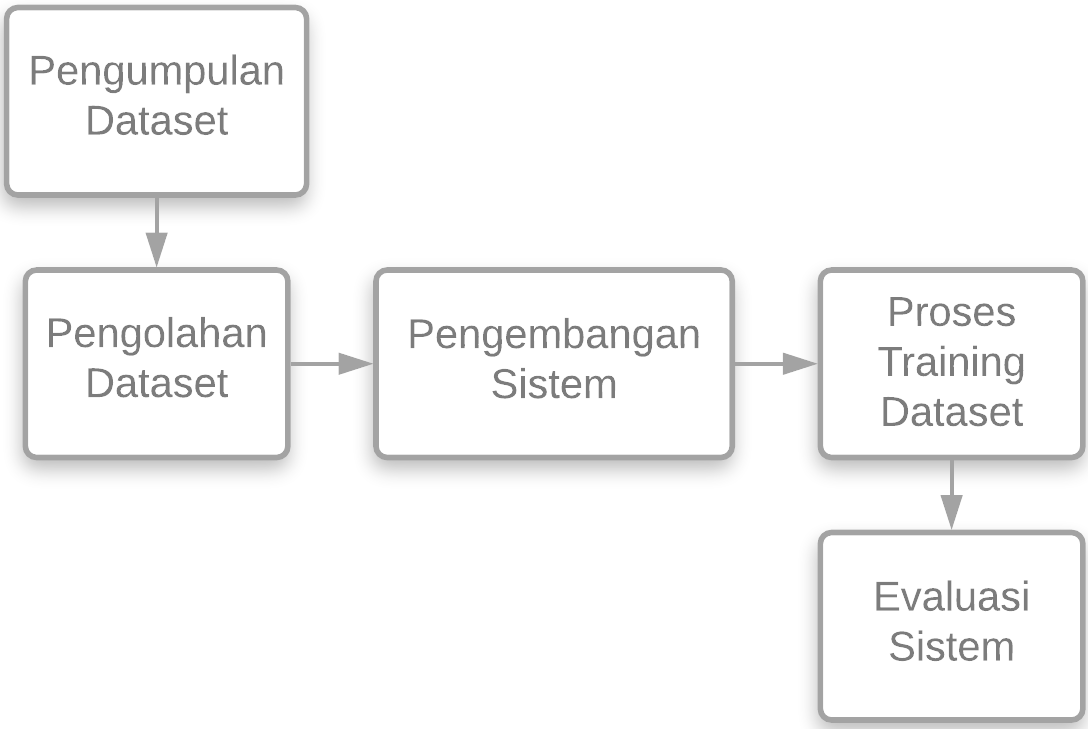
\includegraphics[width=0.7\columnwidth]{gambar/AlurKerja.png}
	
	% Ubah dengan keterangan gambar yang diinginkan
	\caption{Alur Kerja}
	\label{fig:blokdiagram}
\end{figure}

\section{Desain Sistem}
\label{sec:desasinsistem}

Tugas akhir ini merupakan penelitian dalam bidang visi komputer yang bertujuan untuk mendeteksi gerakan mencuci tangan dengan memanfaatkan teknologi \textit{Deep Learning} Berbasis \textit{Convolutional Neural Network (CNN))}. Sistem deteksi ini dilatih menggunakan data training yang diambil dari kaggle (Sample: Handwash Dataset \cite{cit:kaggledata}) ditambahkan dengan dataset yang penulis kumpulkan secara pribadi. 

\section{Alur Kerja}
\label{sec:alurkerja}

Alur implementasi dalam pengerjaan penelitian ini dibagi menjadi beberapa tahapan berdasarkan metodologi penelitian, yaitu: 
\begin{enumerate}[noitemsep]
	\item Pengumpulan Dataset
	\item Pengolahan Dataset
	\item Pengembangan Sistem
	\item Proses Training Dataset
	\item Evaluasi Dataset
\end{enumerate}

\subsection{Pengumpulan Dataset}
\label{subsec:pengumpulandata}

Sebagian besar dataset yang digunakan pada penelitian ini berasal dari Kaggle \cite{cit:kaggledata}. isi dari dataset ini dapat dilihat pada tabel \ref{tab:kagglelist}
% Please add the following required packages to your document preamble:
% \usepackage{graphicx}
\begin{table}[!ht]
	\centering
	\resizebox{0.9\textwidth}{!}{%
		\begin{tabular}{|l|l|c|}
			\hline
			\multicolumn{1}{|c|}{Class} & \multicolumn{1}{c|}{Description}      & \#Videos \\ \hline
			Step 1                      & Rubbing Palm Together                 & 25       \\ \hline
			Step 2 Left                 & Rub Palm Over Dorsum                  & 25       \\ \hline
			Step 2 Right                & Rub Palm Over Dorsum                  & 25       \\ \hline
			Step 3                      & Rubbing Palm With Fingger Interlanced & 25       \\ \hline
			Step 4 Left                 & Rub Nails on Palm                     & 25       \\ \hline
			Step 4 Right                & Rub Nails on Palm                     & 25       \\ \hline
			Step 5 Left                 & Rub Between Thumb and Index Fingger   & 25       \\ \hline
			Step 5 Right                & Rub Between Thumb and Index Fingger   & 25       \\ \hline
			Step 6 Left                 & Rub Finggertips on Palm               & 25       \\ \hline
			Step 6 Right                & Rub Finggertips on Palm               & 25       \\ \hline
			Step 7 Left                 & Rub Thumb                             & 25       \\ \hline
			Step 7 Right                & Rub Thumb                             & 25       \\ \hline
		\end{tabular}%
	}
	\caption{Isi Hand Wash Dataset Kaggle}
	\label{tab:kagglelist}
\end{table}

Pada dataset tersebut, ditemukan berberapa kesalahan seperti kesalahan \textit{labeling}, kesalahan pengelompokan file dan noise berupa video yang \textit{"terkontaminasi"} gerakan berbeda didalamnya, oleh sebab itu dataset ini memerlukan pengecekan dan pemrosesan lebih lanjut agar dapat digunakan pada tahap training. Tidak diketahui spesifikasi kamera yang digunakan dalam pengambilan dataset ini. Sample dari dataset ini dapat dilihat pada gambar \ref{fig:sampledata}

\begin{figure}[!ht]
	\centering
	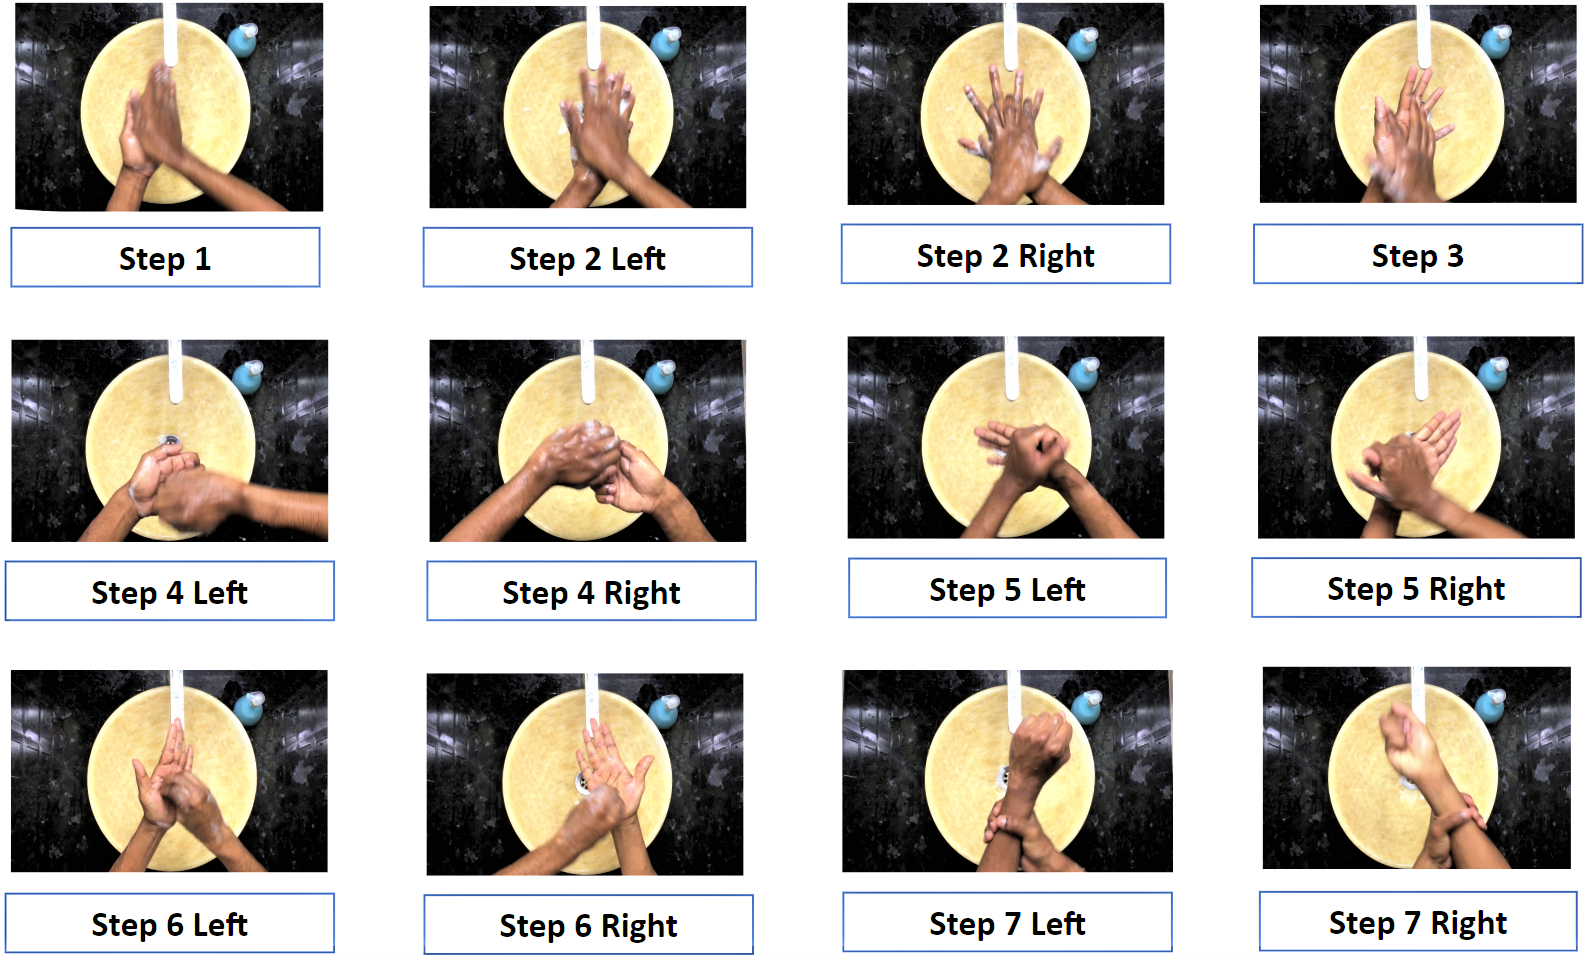
\includegraphics[width=0.9\columnwidth]{gambar/sampledatasetkaggle.png}
	\caption{Sampel dataset Kaggle\cite{cit:kaggledata}}
	\label{fig:sampledata}
\end{figure}

Penulis juga menambahkan dataset pribadi guna melakukan pengujian lebih lanjut. Dataset dikumpulkan dengan 2 kamera berbeda guna mengetahui pengaruh sudut, \textit{background}, serta distorsi lensa pada hasil klasifikasi.

Pengambilan dataset pribadi yang pertama dilakukan di tempat tinggal penulis menggunakan kamera \textit{webcam M-Tech WB-500}. Spesifikasi webcam ini dapat dilihat pada tabel \ref{tab:wb500}
\begin{table}[!ht]
	\centering
	\resizebox{0.6\textwidth}{!}{%
		\begin{tabular}{|l|c|}
			\hline
			\multicolumn{2}{|c|}{Spesifikasi Webcam M-Tech WB-500} \\ \hline
			Maximum Resolution         & 1080p/30fps               \\ \hline
			Image Sensor               & CMOS                      \\ \hline
			Focus Type                 & Fixed Focus               \\ \hline
			Lens                       & 3P                        \\ \hline
			Field of View              & 69°                       \\ \hline
			Microphone                 & Digital                   \\ \hline
			Interface                  & High Speed USB 2.0        \\ \hline
		\end{tabular}%
	}
	\caption{Spesifikasi M-Tech WB-500 \cite{cit:wb500}}
	\label{tab:wb500}
\end{table}

\textit{Setup} pengambilan dataset ini dapat dilihat pada gambar dan contoh video yang didapatkan dapar di lihat pada gambar \ref{fig:webcam2} dan gambar \ref{fig:contohwebcam}

\begin{figure}[!ht]
	\centering
	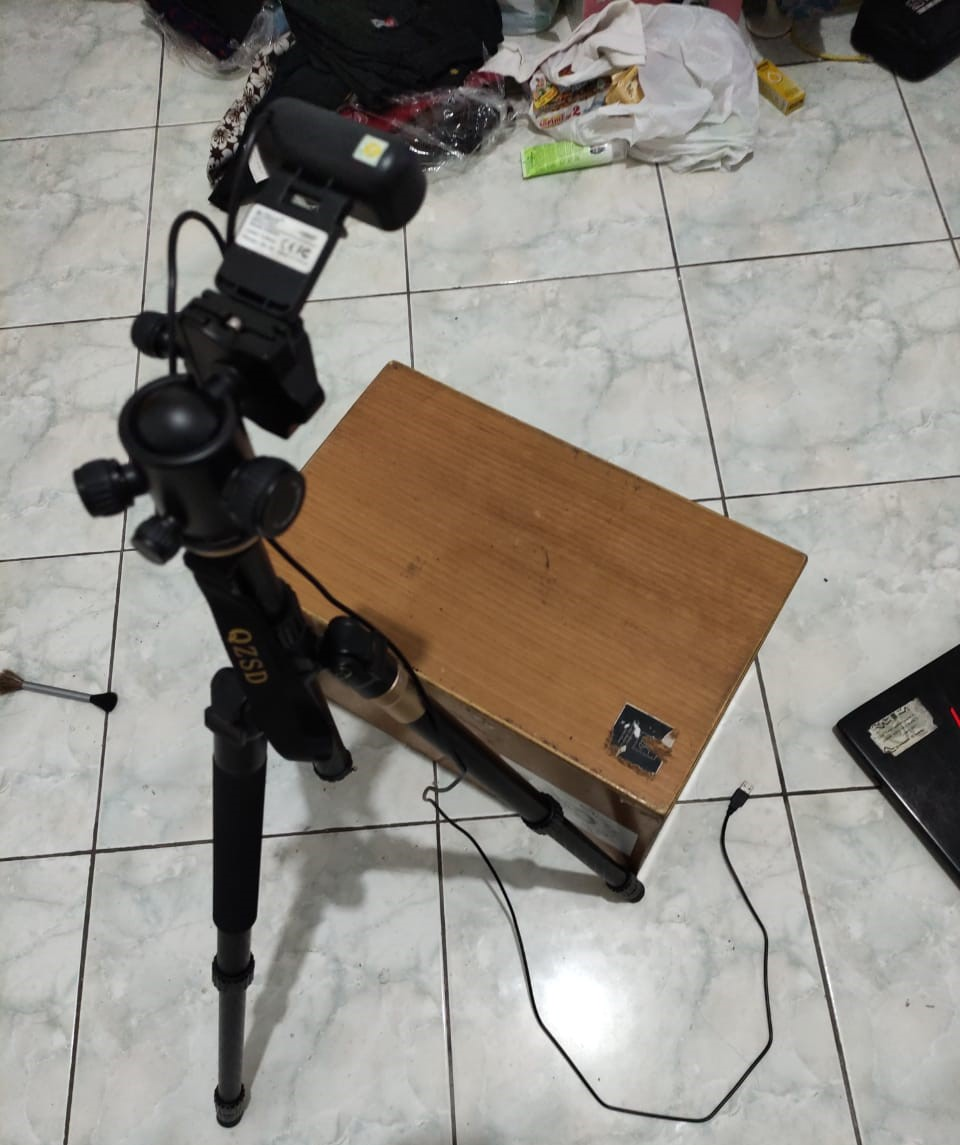
\includegraphics[width=0.7\columnwidth]{gambar/webcam2.jpeg}
	\caption{Setup pengambilan dataset menggunakan webcam}
	\label{fig:webcam2}
\end{figure}

\begin{figure}[!ht]
	\centering
	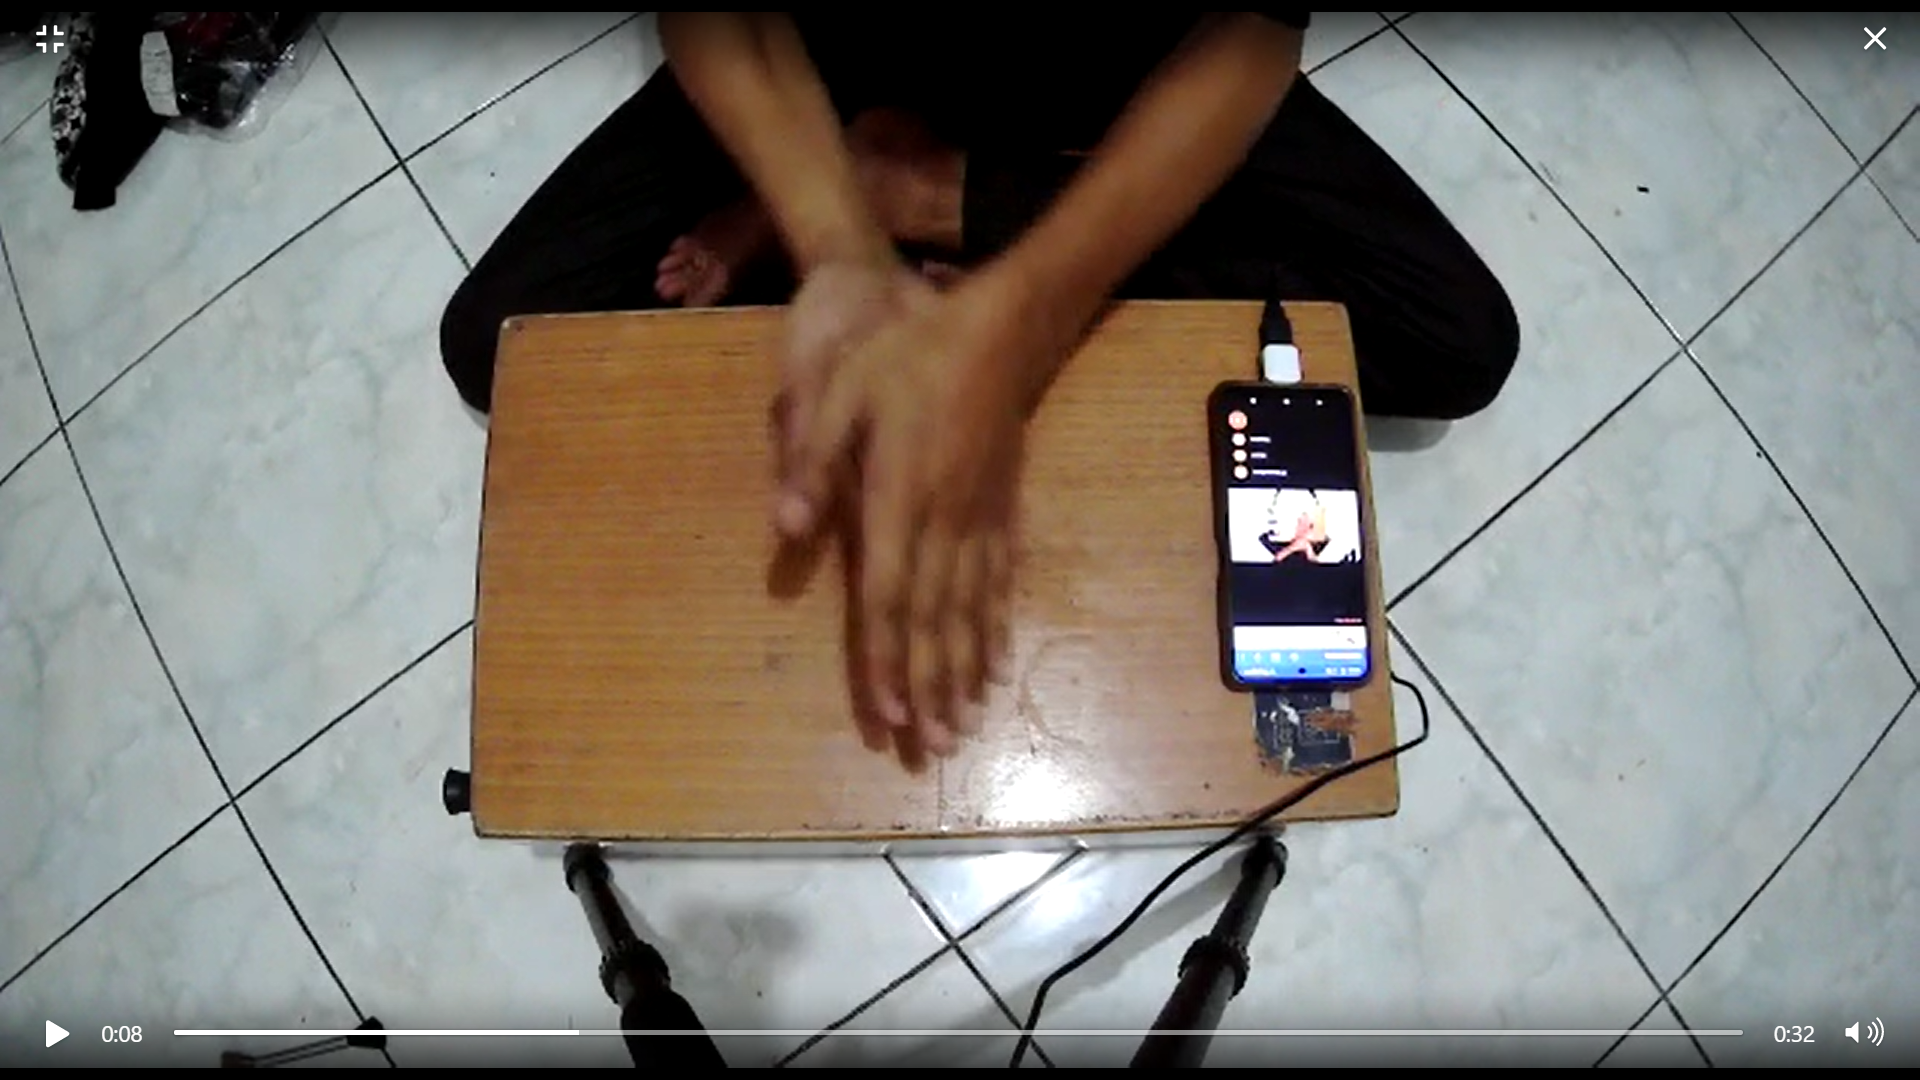
\includegraphics[width=0.8\columnwidth]{gambar/contohwebcam1.png}
	\caption{Contoh hasil video webcam}
	\label{fig:contohwebcam}
\end{figure}

Pengambilan dataset pribadi yang kedua dilakukan di wilayah kampus ITS, tepatnya di gedung laboratorium AJ Elektro. Dataset video ini diambil menggunakan Kamera \textit{DSLR} yang ditempatkan diatas tripod dan diarahkan ke wastafel. Spesifikasi kamera, lensa, dan konfigurasi yang digunakan dapat dilihat pada tabel \ref{tab:canon100d}, \ref{tab:1855stm} dan tabel \ref{tab:pengaturandslr}

\begin{table}[!ht]
	\centering
	\resizebox{0.7\textwidth}{!}{%
		\begin{tabular}{|c|c|}
			\hline
			\multicolumn{2}{|c|}{\textbf{Spesifikasi Dasar Canon EOS 100D}} \\ \hline
			Sensor            & 18 MP APS-C CMOS Sensor                     \\ \hline
			Processor         & DIGIC 5 Image Processor                     \\ \hline
			Display           & 3" 1.04m Dot Clear-View II Touchscreen      \\ \hline
			Video Resolution  & Full HD 1080p Video Recording at 30 fps     \\ \hline
			Auto Focus        & 9-Point AF and Hybrid CMOS AF II            \\ \hline
			ISO               & Native ISO 12800, Extended to ISO 25600     \\ \hline
			Shutter           & 4 fps Shooting for 28 JPEG, 7 Raw Files     \\ \hline
			Metering          & 63-Zone Dual-Layer Metering System          \\ \hline
		\end{tabular}%
	}
	\caption{Spesifikasi Canon EOS 100D \cite{cit:100d}}
	\label{tab:canon100d}
\end{table}

\begin{table}[!ht]
	\centering
	\resizebox{1\textwidth}{!}{%
		\begin{tabular}{|l|l|}
			\hline
			\multicolumn{2}{|c|}{\textbf{Spesifikasi Lensa EF-s 18-55mm f/3.5 - 5.6 IS STM}}                \\ \hline
			Image size                             & APS-C          \\ \hline
			35mm film equivalent focal length (mm) & 29-88          \\ \hline
			Angle of view (horzntl, vertl, diagnl) & 64º 30' - 23º 20', 45º 30'- 15º 40', 74º 20' - 27º 50' \\ \hline
			Lens construction (elements/groups)    & 13/11          \\ \hline
			No. of diaphragm blades                & 7              \\ \hline
			Minimum aperture                       & 22 - 38(36)¹   \\ \hline
			Closest focussing distance (m)         & 0.25           \\ \hline
			Maximum magnification (x)              & 0.36 (at 55mm) \\ \hline
			Distance Information                   & Provided       \\ \hline
			Image stabilizer                       & 4-stops        \\ \hline
			AF actuator                            & STM            \\ \hline
		\end{tabular}%
	}
	\caption{Spesifikasi Lensa EF-s 18-55mm f/3.5 - 5.6 IS STM}
	\label{tab:1855stm}
\end{table}

\begin{table}[!ht]
	\centering
	\resizebox{0.6\textwidth}{!}{%
		\begin{tabular}{|l|l|}
			\hline
			\multicolumn{2}{|c|}{\textbf{Pengaturan Perekaman Kamera DSLR}} \\ \hline
			Resolution                        & 720p 60FPS                  \\ \hline
			Frame Rate                        & 60FPS                       \\ \hline
			Zoom                              & 18mm                        \\ \hline
			Aperture                          & Auto                        \\ \hline
			Focussing                         & Auto Focus                  \\ \hline
			Shutter Speed                     & 60                          \\ \hline
			Image Stablilzer                  & On (Lens)                   \\ \hline
		\end{tabular}%
	}
	\caption{Pengaturan Perekaman Kamera DSLR}
	\label{tab:pengaturandslr}
\end{table}

Setup pengambilan dan contoh hasil video dapat dilihat pada gambar \ref{fig:setupdslr} dan gambar \ref{fig:contohdslr}

\begin{figure}[!ht]
	\centering
	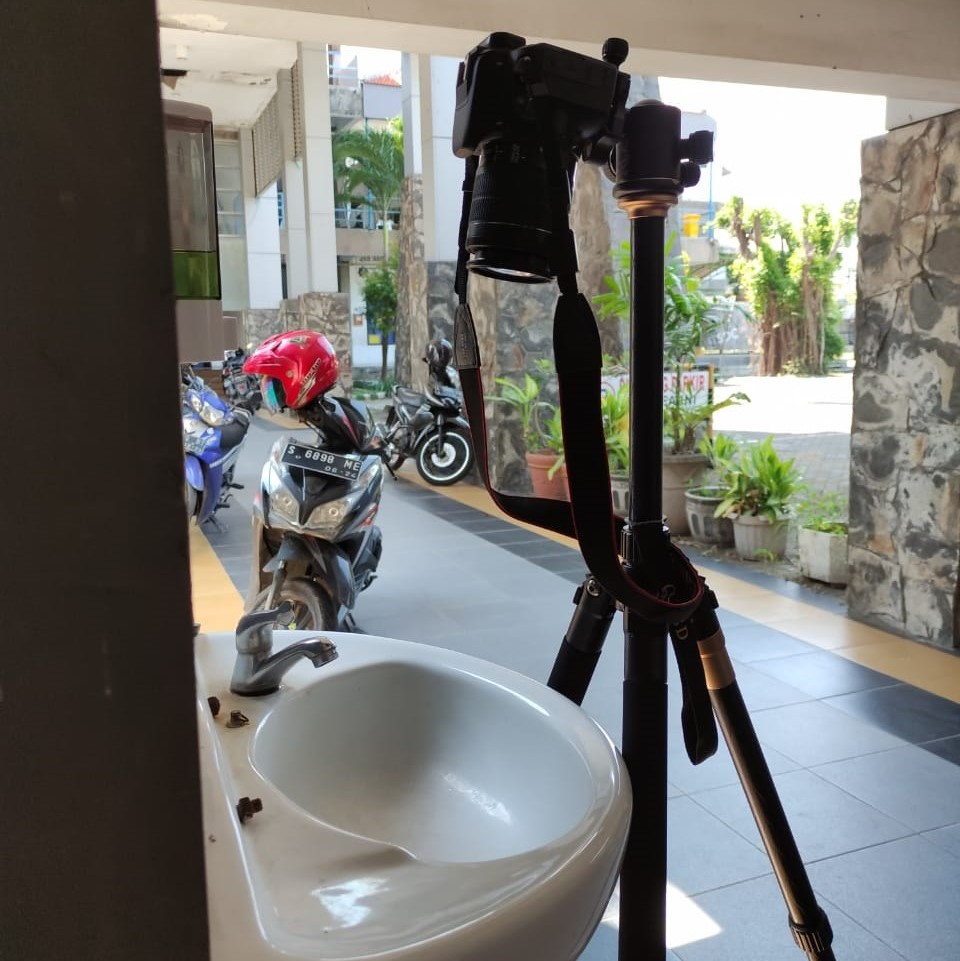
\includegraphics[width=0.6\columnwidth]{gambar/setupdata2.jpeg}
	\caption{Contoh hasil Video DSLR}
	\label{fig:setupdslr}
\end{figure}

\begin{figure}[!ht]
	\centering
	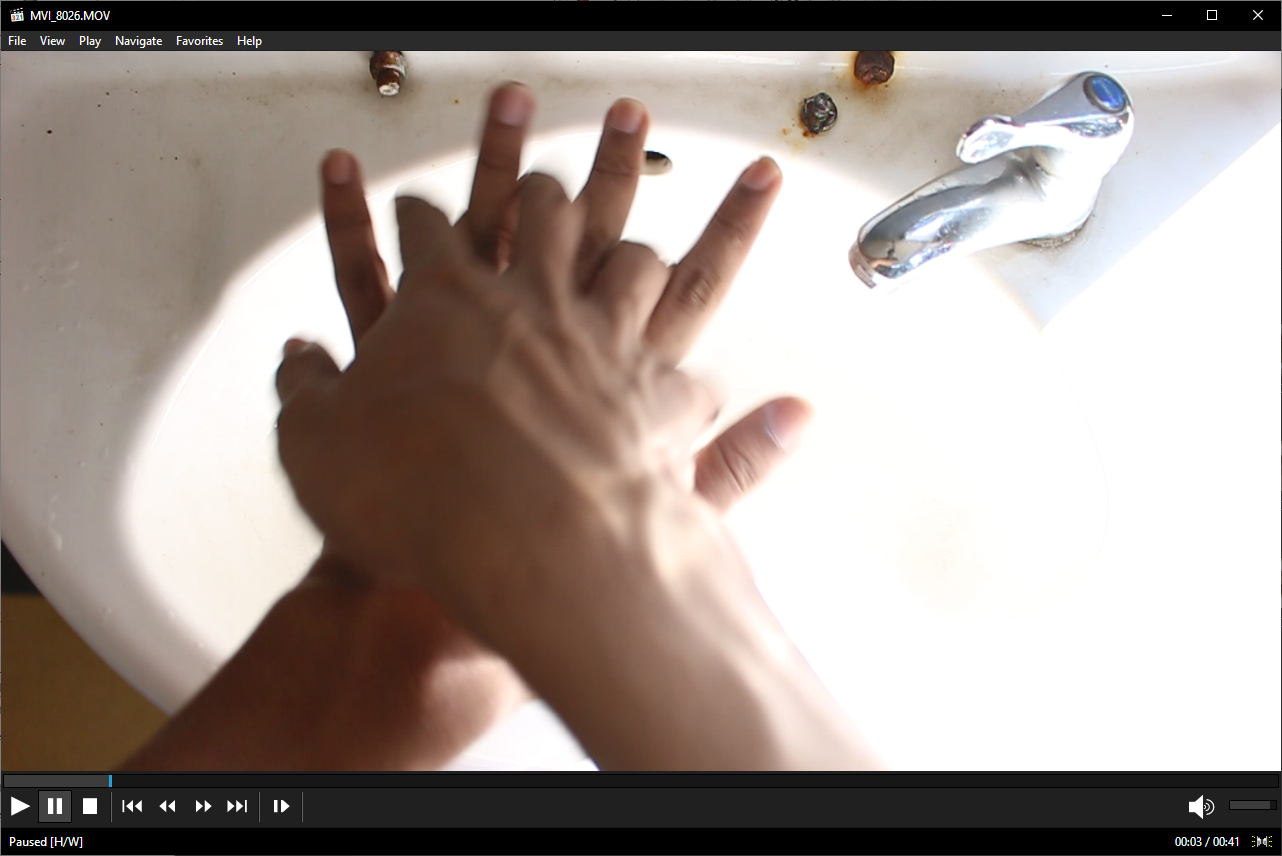
\includegraphics[width=0.8\columnwidth]{gambar/contohdslr2.png}
	\caption{Setup pengambilan dataset menggunakan DSLR}
	\label{fig:contohdslr}
\end{figure}

\subsection{Pengolahan Dataset}
\label{subsec:pengolahandataset}

Pada pengolahan dataset, Dataset yang diambil dari kaggle diperiksa satu-persatu. Pada pemeriksaan ini, ditemukan kesalahan dalam struktural dataset tersebut. Struktur dataset kaggle diperbaiki agar sesuai dengan label nya. berberapa kesalahan pada struktur dataset kaggle ini antara lain gerakan tangan yang tertukar antara kanan dan kiri dan kesalahan peletakan dalam folder. Ditemukan pula kesalahan berupa "kontaminasi" gerakan yang berbeda pada satu video gerakan. Hal ini kemudian diperbaiki dengan membuang kontaminasi tersebut

Dataset yang diambil secara pribadi dari Webcam dan DSLR juga diperiksa. kontaminasi juga ditemukan akibat ketidaksengajaan pada proses perekaman dan turut dibersihkan. kemudian berberapa video dengan durasi yang terlalu lama di potong menjadi 2 video terpisah. Dataset ini kemudian di \textit{encoding} ulang untuk mempermudah proses training.

\subsection{Training}
\label{subsec:trainigg}

\
% Contoh input potongan kode dari file
\lstinputlisting[
  language=Python,
  caption={Program perhitungan bilangan prima.},
  label={lst:bilanganprima}
]{program/bilangan-prima.py}

